\documentclass[aspectratio=169,11pt]{beamer}
% =====================================================================
%  Acute Netrin-1 RNA-seq — Thesis defense (~35 min)
%  Compile: pdflatex thesis_defense.tex  (run twice for the outline)
% =====================================================================
\usepackage[utf8]{inputenc}
\usepackage{booktabs}
\usepackage{colortbl}
\usepackage{array}
\usepackage{tikz}
\usetikzlibrary{arrows.meta,positioning,calc}
\usepackage{graphicx}
\graphicspath{{../assets/}}

% ---------- theme ----------------------------------------------------
\usetheme{default}
\usefonttheme{professionalfonts}
\setbeamertemplate{navigation symbols}{}

\definecolor{navy}{HTML}{102A43}
\definecolor{teal}{HTML}{16828C}
\definecolor{teald}{HTML}{0E5A61}
\definecolor{greyt}{HTML}{444A52}
\definecolor{lgrey}{HTML}{6B727B}
\definecolor{reddn}{HTML}{C0392B}
\definecolor{grnup}{HTML}{1E7D52}
\definecolor{lbg}{HTML}{F3F6F7}
\definecolor{abg}{HTML}{EAF3F3}

\setbeamercolor{structure}{fg=teal}
\setbeamercolor{frametitle}{fg=navy}
\setbeamercolor{normal text}{fg=greyt}
\setbeamercolor{itemize item}{fg=teal}
\setbeamercolor{itemize subitem}{fg=teald}
\setbeamerfont{frametitle}{series=\bfseries,size=\large}
\setbeamertemplate{itemize item}{\raisebox{0.15ex}{\footnotesize$\blacktriangleright$}}
\setbeamertemplate{itemize subitem}{\textendash}

% frame title with accent rule
\setbeamertemplate{frametitle}{%
  \vskip6pt
  {\color{teal}\footnotesize\bfseries\MakeUppercase{\insertframesubtitle}}\par
  \vskip1pt
  {\color{navy}\large\bfseries\insertframetitle}\par
  \vskip2pt{\color{teal}\rule{2.2em}{1.6pt}}\par
}
\setbeamertemplate{footline}{%
  \hfill{\color{lgrey}\scriptsize\insertframenumber}\hspace{2ex}\vskip4pt}

\newcommand{\up}{\textcolor{grnup}{\textbf{up}}}
\newcommand{\dn}{\textcolor{reddn}{\textbf{down}}}
\newcommand{\hi}[1]{\textcolor{navy}{\textbf{#1}}}
\newcommand{\tl}[1]{\textcolor{teald}{\textbf{#1}}}

% =====================================================================
\begin{document}

% ---------- TITLE ----------------------------------------------------
{\setbeamertemplate{footline}{}
\begin{frame}[plain]
  \begin{tikzpicture}[remember picture,overlay]
    \fill[navy] (current page.south west) rectangle (current page.north east);
    \fill[teal] ([yshift=-2.7cm]current page.west) rectangle ([yshift=-2.62cm]current page.east);
  \end{tikzpicture}
  \vskip1.2cm
  {\color{teal!50!white}\small\bfseries ACUTE TRANSCRIPTIONAL RESPONSE $\cdot$ BULK RNA-SEQ TIME COURSE}\par
  \vskip10pt
  {\color{white}\Large\bfseries A Rapid, Coordinated and Transient\\[2pt]
   Transcriptional Program Triggered by\\[2pt]
   \color{teal!70!white}Acute Netrin-1 Stimulation in Cortical Neurons}\par
  \vskip28pt
  {\color{white!85!navy}\itshape 5- and 15-minute Netrin-1 time course in E18 rat cortical neurons}\par
  \vskip22pt
  {\color{white}\small\bfseries Thesis Defense}\par
  {\color{white!60!navy}\footnotesize [ Your name ] $\cdot$ [ Department / Institution ] $\cdot$ [ Date ]}\par
\end{frame}}

% ---------- OUTLINE --------------------------------------------------
\begin{frame}
  \frametitle{Outline}\framesubtitle{Roadmap}
  \begin{columns}[T]
    \begin{column}{0.6\textwidth}
      \begin{itemize}\setlength\itemsep{4pt}
        \item Background --- Netrin-1 and the gap in acute transcription
          \begin{itemize}\item Why look at minutes, not hours?\end{itemize}
        \item Question, hypothesis \& experimental design
        \item Analysis pipeline \& quality control
        \item Results
          \begin{itemize}
            \item 1 $\cdot$ The 5-minute response (genes)
            \item 2 $\cdot$ Transient dynamics (IEGs, ROCK1)
            \item 3 $\cdot$ Pathway-level coordination (GSEA)
            \item 4 $\cdot$ Return to baseline --- the $r=-0.99$ mirror
          \end{itemize}
        \item Discussion, limitations \& conclusions
      \end{itemize}
    \end{column}
    \begin{column}{0.38\textwidth}
      \colorbox{lbg}{\parbox{\textwidth}{\vskip2pt
        {\color{teald}\scriptsize\bfseries THE ONE-SENTENCE STORY}\\[3pt]
        \small A 5-min Netrin-1 pulse activates an axon-guidance / projection
        program and suppresses RNA-processing \& ribosome biogenesis --- then by
        15 min returns to baseline with $r=-0.99$ precision.\vskip3pt}}
    \end{column}
  \end{columns}
  \note{~1 min. Roadmap. First third = context + methods; middle = four result
  blocks; close = discussion. Remember the box: a transient program switched on
  then precisely off within 15 minutes.}
\end{frame}

% ---------- BACKGROUND 1 ---------------------------------------------
\begin{frame}
  \frametitle{Netrin-1: a classic guidance cue --- acting in seconds}\framesubtitle{Background}
  \begin{columns}[T]
    \begin{column}{0.56\textwidth}
      \begin{itemize}\setlength\itemsep{6pt}
        \item \hi{Netrin-1 is a prototypical axon-guidance molecule.}
          \begin{itemize}\item Steers the growth cone via DCC and UNC5 receptors.\end{itemize}
        \item \hi{Canonical mechanism is POST-translational and LOCAL.}
          \begin{itemize}
            \item Cytoskeletal remodeling, local translation.
            \item Seconds-to-minutes timescale.
          \end{itemize}
        \item \hi{The field focuses on protein-level signaling\ldots}
          \begin{itemize}\item \ldots and overlooks the nucleus on this timescale.\end{itemize}
      \end{itemize}
    \end{column}
    \begin{column}{0.42\textwidth}
      \colorbox{lbg}{\parbox{\textwidth}{\centering\vskip3pt
        {\color{teald}\scriptsize\bfseries CANONICAL NETRIN-1 SIGNALING}\\[6pt]
        {\color{navy}\bfseries Netrin-1}\\[2pt]{\color{teal}$\downarrow$}\\[2pt]
        DCC / UNC5 receptors\\[2pt]{\color{teal}$\downarrow$}\\[2pt]
        Cytoskeleton $\cdot$ ROCK $\cdot$ local translation\\[2pt]{\color{teal}$\downarrow$}\\[2pt]
        {\color{navy}\bfseries Growth-cone turning}\\{\footnotesize(seconds--minutes)}\vskip4pt}}
    \end{column}
  \end{columns}
  \note{~1.5 min. Netrin-1 is the textbook cue; binds DCC/UNC5, steers the growth
  cone. Classic mechanism is post-translational and local, seconds-minutes. So the
  field overlooks what the nucleus does on this fast timescale --- the door this
  thesis opens.}
\end{frame}

% ---------- BACKGROUND 2 / GAP ---------------------------------------
\begin{frame}
  \frametitle{The knowledge gap: minutes-scale transcription}\framesubtitle{Background}
  \begin{center}
  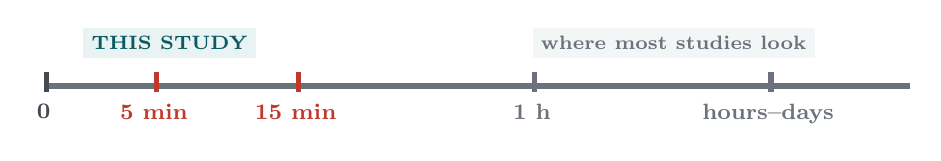
\begin{tikzpicture}[font=\small]
    \draw[lgrey,line width=2pt] (0,0)--(11,0);
    \foreach \x/\lab/\c in {0/0/greyt,1.4/{5 min}/reddn,3.2/{15 min}/reddn,6.2/{1 h}/lgrey,9.2/{hours--days}/lgrey}{
      \fill[\c] (\x,-0.08) rectangle (\x+0.07,0.18);
      \node[\c,font=\footnotesize\bfseries,below=3pt] at (\x,0) {\lab};}
    \node[teald,font=\scriptsize\bfseries,fill=abg,inner sep=3pt] at (1.6,0.55) {THIS STUDY};
    \node[lgrey,font=\scriptsize\bfseries,fill=lbg,inner sep=3pt] at (8.0,0.55) {where most studies look};
  \end{tikzpicture}
  \end{center}
  \vskip6pt
  \begin{itemize}\setlength\itemsep{7pt}
    \item Almost all Netrin transcriptome studies sample \textbf{hours to days} after stimulation.
    \item \hi{The acute, minute-scale transcriptional response is essentially uncharted.}
    \item Open questions: does the transcriptome change within minutes? \emph{How}?
      And is the change \emph{transient} or \emph{sustained}?
  \end{itemize}
  \note{~1.5 min. Timeline: studies cluster at hours-days (right); the 5/15-min
  window is blank. Three questions: does it change in minutes? how? transient or
  sustained? These define the thesis.}
\end{frame}

% ---------- QUESTION & HYPOTHESIS ------------------------------------
\begin{frame}
  \frametitle{Research question \& hypothesis}\framesubtitle{Aim}
  \begin{beamercolorbox}[wd=\textwidth,sep=8pt]{}
  \colorbox{navy}{\parbox{0.97\textwidth}{\color{white}
    {\color{teal!60!white}\footnotesize\bfseries RESEARCH QUESTION}\\[3pt]
    \large\bfseries Does acute Netrin-1 stimulation rapidly reshape the neuronal
    transcriptome --- and is that response transient or persistent?}}
  \end{beamercolorbox}
  \vskip8pt
  \begin{columns}[T]
    \begin{column}{0.48\textwidth}
      \colorbox{lbg}{\parbox{\textwidth}{\vskip2pt
        {\color{teal}\scriptsize\bfseries HYPOTHESIS}\\[4pt]
        \small Netrin-1 induces a fast, coordinated transcriptional response \ldots
        that is \tl{transient} --- switched on, then off --- rather than a stable
        reprogramming.\vskip3pt}}
    \end{column}
    \begin{column}{0.48\textwidth}
      \colorbox{abg}{\parbox{\textwidth}{\vskip2pt
        {\color{teald}\scriptsize\bfseries APPROACH}\\[4pt]
        \small Bulk RNA-seq time course 0/5/15 min $\cdot$ DESeq2 differential
        expression $\cdot$ GSEA pathway coordination $\cdot$ compare 5v0 vs 15v5 to
        test reversibility.\vskip3pt}}
    \end{column}
  \end{columns}
  \note{~1.5 min. Question stated plainly; hypothesis = fast, coordinated,
  transient. Approach: 0/5/15 time course, DESeq2, GSEA. Key reversibility test =
  5v0 vs 15v5 mirror --- pays off at the end.}
\end{frame}

% ---------- EXPERIMENTAL DESIGN --------------------------------------
\begin{frame}
  \frametitle{Experimental design}\framesubtitle{Methods}
  \begin{columns}[T]
    \begin{column}{0.55\textwidth}
      \begin{itemize}\setlength\itemsep{5pt}
        \item \hi{E18 rat cortical mixed primary cultures.}
        \item \hi{Three conditions:}
          \begin{itemize}
            \item Vehicle (PBS, 5 min) --- reference / 0 min
            \item Netrin-1, 5 min \quad $\cdot$\quad Netrin-1, 15 min
          \end{itemize}
        \item \hi{3 biological replicates $\rightarrow$ 9 samples.}
        \item \textcolor{reddn}{\textbf{Design limitation:}} one shared PBS-5min
          control serves \emph{both} Netrin timepoints --- no independent PBS-15min.
          \begin{itemize}\item[\textcolor{reddn}{$\rightarrow$}]
            \textcolor{reddn}{confounds 15v0; main results use 5v0 and 15v5.}\end{itemize}
      \end{itemize}
    \end{column}
    \begin{column}{0.43\textwidth}
      \colorbox{lbg}{\parbox{\textwidth}{\centering\vskip3pt
        {\color{teald}\scriptsize\bfseries 9 SAMPLES = 3 COND.\ $\times$ 3 REP.}\\[5pt]
        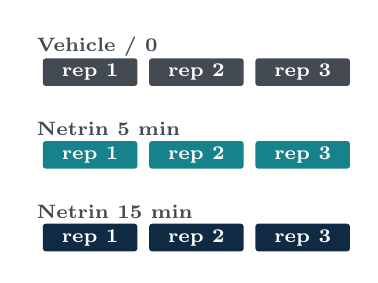
\begin{tikzpicture}[font=\scriptsize\bfseries\color{white},
            box/.style={rounded corners=1pt,minimum width=1.2cm,minimum height=0.5cm}]
          \foreach \r/\c/\lab in {0/greyt/{Vehicle / 0},1/teal/{Netrin 5 min},2/navy/{Netrin 15 min}}{
            \node[greyt,font=\scriptsize\bfseries,anchor=west] at (-0.2,-1.05*\r+0.25) {\lab};
            \foreach \k in {0,1,2}{\fill[\c,rounded corners=1pt] (1.35*\k,-1.05*\r-0.25) rectangle (1.35*\k+1.2,-1.05*\r+0.1);
              \node at (1.35*\k+0.6,-1.05*\r-0.08){rep \the\numexpr\k+1\relax};}}
        \end{tikzpicture}\vskip3pt}}
    \end{column}
  \end{columns}
  \note{~1.5 min. E18 cortical cultures, 3 conditions, 3 reps, 9 samples. Flag up
  front: ONE shared PBS-5min control for both timepoints, no 15-min vehicle ---
  confounds 15v0 with elapsed time, so main results use 5v0 and 15v5.}
\end{frame}

% ---------- PIPELINE -------------------------------------------------
\begin{frame}
  \frametitle{Analysis pipeline}\framesubtitle{Methods}
  \begin{center}
  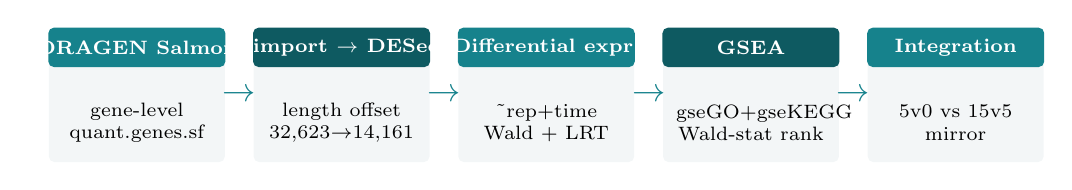
\begin{tikzpicture}[font=\scriptsize,node distance=2pt,
      box/.style={rounded corners=2pt,draw=none,text width=2.0cm,align=center,
        minimum height=1.7cm,fill=lbg},
      hd/.style={font=\scriptsize\bfseries\color{white}}]
    \node[box](a){}; \node[box,right=10pt of a](b){};
    \node[box,right=10pt of b](c){}; \node[box,right=10pt of c](d){};
    \node[box,right=10pt of d](e){};
    \foreach \n/\t/\col in {a/{DRAGEN Salmon}/teal,b/{tximport $\to$ DESeq2}/teald,
        c/{Differential expr.}/teal,d/{GSEA}/teald,e/{Integration}/teal}{
      \fill[\col,rounded corners=2pt] (\n.north west) rectangle ([yshift=-0.5cm]\n.north east);
      \node[hd] at ([yshift=-0.25cm]\n.north){\t};}
    \node[align=center,text width=1.9cm] at ([yshift=-0.35cm]a.center){gene-level\\ quant.genes.sf};
    \node[align=center,text width=1.9cm] at ([yshift=-0.35cm]b.center){length offset\\ 32{,}623$\to$14{,}161};
    \node[align=center,text width=1.9cm] at ([yshift=-0.35cm]c.center){\textasciitilde rep+time\\ Wald + LRT};
    \node[align=center,text width=1.9cm] at ([yshift=-0.35cm]d.center){gseGO+gseKEGG\\ Wald-stat rank};
    \node[align=center,text width=1.9cm] at ([yshift=-0.35cm]e.center){5v0 vs 15v5\\ mirror};
    \foreach \x/\y in {a/b,b/c,c/d,d/e}{\node[teal,font=\large\bfseries] at ($(\x)!0.5!(\y)$){$\to$};}
  \end{tikzpicture}
  \end{center}
  \vskip8pt
  \small Quantification with DRAGEN Salmon (gene level); counts imported via
  tximport with a length offset into DESeq2. Two-pass filtering keeps
  \hi{14{,}161 of 32{,}623} genes (85.6\% SYMBOL-mapped). Replicate is a batch term;
  \tl{batch correction is for visualization only --- DE tests use raw counts.}
  \note{~1.5 min. Five steps: Salmon quant, DESeq2 import, DE, GSEA, integration.
  Filtering 32.6k$\to$14.2k, ~86\% symbol-mapped. Batch correction visualization-only;
  tests on raw counts with batch term.}
\end{frame}

% ---------- METHODS DETAIL -------------------------------------------
\begin{frame}
  \frametitle{Statistical model \& significance}\framesubtitle{Methods}
  \begin{columns}[T]
    \begin{column}{0.49\textwidth}
      \colorbox{teal}{\color{white}\scriptsize\bfseries\ \ DIFFERENTIAL EXPRESSION\ \ }\\[4pt]
      \footnotesize
      \begin{itemize}\setlength\itemsep{3pt}
        \item Model: \texttt{\textasciitilde\ replicate + timepoint} (ref = Vehicle).
        \item Replicate dominates variance: PCA \hi{rep $\approx$52\%, time $\approx$34\%}.
        \item Wald: 5v0, 15v0, 15v5; LRT (reduced \texttt{\textasciitilde rep}).
        \item \textbf{RELAXED}: padj $<$ 0.05.
        \item \textbf{STRICT}: padj $<$ 0.05 \& $|$log2FC$|>$0.585 (FC$>$1.5).
      \end{itemize}
    \end{column}
    \begin{column}{0.49\textwidth}
      \colorbox{teald}{\color{white}\scriptsize\bfseries\ \ GENE-SET ENRICHMENT (GSEA)\ \ }\\[4pt]
      \footnotesize
      \begin{itemize}\setlength\itemsep{3pt}
        \item clusterProfiler gseGO(BP) + gseKEGG (rno).
        \item Rank = DESeq2 Wald stat; entrez de-dup (max $|$stat$|$).
        \item minGSSize 15 $\cdot$ maxGSSize 500 $\cdot$ BH $\cdot$ seed 123.
        \item GO simplified (0.7) to drop redundancy.
        \item \hi{Why GSEA: acute signal weak per-gene --- pathway aggregation
          reveals the coordinated program.}
      \end{itemize}
    \end{column}
  \end{columns}
  \note{~1.5 min. DE: model rep+time, rep dominates (52 vs 34\%), two sig tiers.
  GSEA ranked by Wald stat. Key: signal weak per-gene, so pathway-level GSEA is the
  primary analysis.}
\end{frame}

% ---------- QC 1: composition ----------------------------------------
\begin{frame}
  \frametitle{Quality control I --- neuron-dominated \& stable}\framesubtitle{Results $\cdot$ QC}
  \begin{columns}[c]
    \begin{column}{0.55\textwidth}\centering
      \includegraphics[height=0.78\textheight]{f_composition.png}\end{column}
    \begin{column}{0.43\textwidth}\footnotesize
      \begin{itemize}\setlength\itemsep{6pt}
        \item \hi{Pan-neuronal markers dominate:} Tubb3 $\approx$3900, Stmn2
          $\approx$1540, Map2 $\approx$750 TPM.
          \begin{itemize}\item 2--4 orders above glial/endothelial (Vwf, Flt1 $\approx$0.1).\end{itemize}
        \item \tl{Marker profile near-identical across all 3 conditions.}
          \begin{itemize}\item[$\rightarrow$] cell composition does \emph{not} change.\end{itemize}
        \item \hi{Downstream changes = genuine transcriptional response, not a
          shift in cell types.}
      \end{itemize}
    \end{column}
  \end{columns}
  \note{~1.5 min. Neuron-dominated cultures (markers hundreds-thousands TPM vs ~0.1
  for glia/endo). Profile identical across conditions --- 5/15 min too short to
  change composition. So downstream = real transcriptional response.}
\end{frame}

% ---------- QC 2: PCA ------------------------------------------------
\begin{frame}
  \frametitle{Quality control II --- replicate is the top batch effect}\framesubtitle{Results $\cdot$ QC}
  \begin{columns}[c]
    \begin{column}{0.6\textwidth}\centering
      \includegraphics[height=0.78\textheight]{f_pca_after.png}\end{column}
    \begin{column}{0.38\textwidth}\footnotesize
      \begin{itemize}\setlength\itemsep{6pt}
        \item \textcolor{reddn}{\textbf{Top variation = biological REPLICATE, not treatment}}
          (rep $\approx$52\%, time $\approx$34\%).
        \item Handled: replicate a batch term; limma removeBatchEffect for
          visualization only.
        \item \tl{After correction, PC1 mainly reflects TIMEPOINT} --- samples
          separate by 0/5/15 min.
      \end{itemize}
    \end{column}
  \end{columns}
  \note{~1.5 min. Largest variance = replicate, not treatment (52 vs 34\%). So
  replicate is a batch term. PCA shown after correction (viz only); PC1 now aligns
  with timepoint. Stats still on raw counts.}
\end{frame}

% ---------- R1 volcano -----------------------------------------------
\begin{frame}
  \frametitle{Result 1 --- the 5-minute response is real but small}\framesubtitle{Results $\cdot$ DEGs}
  \begin{columns}[c]
    \begin{column}{0.58\textwidth}\centering
      \includegraphics[height=0.8\textheight]{f_volcano.png}\end{column}
    \begin{column}{0.4\textwidth}\footnotesize
      \begin{itemize}\setlength\itemsep{5pt}
        \item \hi{5v0:} RELAXED \textbf{32} (14$\uparrow$/18$\downarrow$);
          STRICT \textbf{5} (2$\uparrow$/3$\downarrow$).
        \item \textcolor{reddn}{\textbf{Fos} stands out:} log2FC $-2.35$,
          padj 2.4e\textendash3 --- strongly down.
        \item Most effects modest --- a fast, subtle, pathway-level signal.
        \item[\tl{$\rightarrow$}] \tl{motivates the GSEA analysis.}
      \end{itemize}
    \end{column}
  \end{columns}
  \note{~1.5 min. 5v0 volcano: 32 DEGs relaxed, 5 strict. Outlier = Fos, down >4x
  (direction surprising --- return to it). Real but small per-gene; motivates GSEA.}
\end{frame}

% ---------- R1 table -------------------------------------------------
\begin{frame}
  \frametitle{Core 5-minute DEGs map onto coherent modules}\framesubtitle{Results $\cdot$ DEGs}
  \centering\small
  \renewcommand{\arraystretch}{1.25}
  \begin{tabular}{>{\bfseries\color{navy}}l c c l}
    \toprule
    \rowcolor{navy}\textbf{\color{white}Gene} & \textbf{\color{white}log2FC}
      & \textbf{\color{white}padj} & \textbf{\color{white}Module}\\
    \midrule
    Fos & \textcolor{reddn}{\textbf{$-2.35$}} & 2.4e\textendash3 & \textcolor{reddn}{Immediate-early gene (IEG $\downarrow$)}\\
    Rock1 & \textcolor{reddn}{\textbf{$-0.43$}} & 9.4e\textendash6 & \textcolor{reddn}{Cytoskeleton / ROCK}\\
    Srsf5 & \textcolor{reddn}{\textbf{$-0.31$}} & 4.5e\textendash5 & \textcolor{reddn}{Splicing}\\
    Snrnp70 & \textcolor{reddn}{\textbf{$-0.27$}} & 1.2e\textendash2 & \textcolor{reddn}{Splicing}\\
    Cntn2 & \textcolor{grnup}{\textbf{$+0.25$}} & 1.4e\textendash2 & \textcolor{grnup}{Axon guidance}\\
    Nos1 & \textcolor{grnup}{\textbf{$+0.32$}} & 3.5e\textendash2 & \textcolor{grnup}{NO--calcium}\\
    Ryr3 & \textcolor{grnup}{\textbf{$+0.47$}} & 2.4e\textendash2 & \textcolor{grnup}{NO--calcium}\\
    Tln2 & \textcolor{grnup}{\textbf{$+0.39$}} & 1.2e\textendash2 & \textcolor{grnup}{Adhesion}\\
    \bottomrule
  \end{tabular}\par\vskip8pt
  \footnotesize\itshape Down: IEG, cytoskeleton, splicing. \quad Up: axon guidance,
  NO--calcium, adhesion. \quad Small individually --- but clean, interpretable modules.
  \note{~1.5 min. The genes sort into modules. Down: Fos (IEG), Rock1
  (cytoskeleton), Srsf5/Snrnp70 (splicing). Up: Cntn2 (guidance), Nos1/Ryr3
  (NO-calcium), Tln2 (adhesion). Small but coherent --- preview of GSEA.}
\end{frame}

% ---------- R2 trajectory --------------------------------------------
\begin{frame}
  \frametitle{Result 2 --- a transient 5-minute pulse}\framesubtitle{Results $\cdot$ Dynamics}
  \begin{columns}[c]
    \begin{column}{0.6\textwidth}\centering
      \includegraphics[height=0.78\textheight]{f_traj.png}\end{column}
    \begin{column}{0.38\textwidth}\footnotesize
      \begin{itemize}\setlength\itemsep{6pt}
        \item \hi{LRT: 19 genes change significantly over time.}
        \item \tl{Dominant shape = a 5-min PULSE:} depart at 5 min, return by 15.
        \item \hi{First direct evidence the program is transient, not sustained.}
        \item \textcolor{reddn}{Caveat:} Fos at 15 min overshoots baseline; variable
          Vehicle replicates $\rightarrow$ wide error band.
      \end{itemize}
    \end{column}
  \end{columns}
  \note{~1.5 min. LRT flags 19 time-varying genes; dominant shape = pulse
  (depart@5, return@15) --- first direct evidence of transience. Caveat: Fos
  overshoots at 15, noisy vehicle reps, wide band.}
\end{frame}

% ---------- R2 IEG ---------------------------------------------------
\begin{frame}
  \frametitle{A surprise: two immediate-early genes are SUPPRESSED}\framesubtitle{Results $\cdot$ Dynamics}
  \colorbox{abg}{\parbox{0.97\textwidth}{\vskip2pt\color{navy}\bfseries
    Immediate-early genes are normally \emph{activated} by neuronal activity. Here,
    acute Netrin-1 does the opposite --- it acutely DOWN-regulates them.\vskip2pt}}
  \vskip10pt
  \begin{columns}[T]
    \begin{column}{0.48\textwidth}
      \colorbox{lbg}{\parbox{\textwidth}{\vskip3pt
        {\color{reddn}\Large\bfseries Fos}\\[3pt]
        log2FC $-2.35$ $\cdot$ padj 2.4e\textendash3\\
        \itshape The strongest DEG of the study.\\[4pt]
        \hi{Strong, significant acute repression.}\vskip3pt}}
    \end{column}
    \begin{column}{0.48\textwidth}
      \colorbox{lbg}{\parbox{\textwidth}{\vskip3pt
        {\color{reddn}\Large\bfseries Npas4}\\[3pt]
        log2FC $-1.75$ $\cdot$ padj 0.076 (Wald, n.s.)\\
        \itshape Significant by the time-course LRT.\\[4pt]
        \hi{A second acutely-repressed IEG.}\vskip3pt}}
    \end{column}
  \end{columns}
  \note{~1.5 min. IEGs normally go UP with activity; here Fos and Npas4 both go
  DOWN. Fos >4x down, strongest DEG. Npas4 ~3.4x down, n.s. by Wald but sig by LRT.
  Two independent IEGs repressed --- novel, counterintuitive.}
\end{frame}

% ---------- R2 ROCK --------------------------------------------------
\begin{frame}
  \frametitle{Selective control: Rock1 down, Rock2 untouched}\framesubtitle{Results $\cdot$ Dynamics}
  \begin{columns}[c]
    \begin{column}{0.6\textwidth}\centering
      \includegraphics[height=0.78\textheight]{f_rock.png}\end{column}
    \begin{column}{0.38\textwidth}\footnotesize
      \begin{itemize}\setlength\itemsep{7pt}
        \item \textcolor{reddn}{\textbf{Rock1}: log2FC $-0.43$, padj 9.4e\textendash6 --- down.}
        \item \textcolor{lgrey}{\textbf{Rock2}: log2FC $+0.07$, padj $\approx$1.0 --- unchanged.}
        \item \hi{Two paralogues, opposite fates in one cell.}
        \item ROCK1 is a classic Netrin--DCC effector.
        \item[\tl{$\rightarrow$}] \tl{isoform-selective transcriptional control --- precise, not blunt.}
      \end{itemize}
    \end{column}
  \end{columns}
  \note{~1.5 min. Rock1 down (padj ~1e-5), Rock2 unchanged --- same cell, same
  family, opposite fates. ROCK1 is canonical Netrin-DCC effector. Response is
  selective, not blunt.}
\end{frame}

% ---------- heatmap --------------------------------------------------
\begin{frame}
  \frametitle{DEGs separate the conditions coherently}\framesubtitle{Results $\cdot$ Dynamics}
  \begin{columns}[c]
    \begin{column}{0.5\textwidth}\centering
      \includegraphics[height=0.8\textheight]{f_heatmap.png}\end{column}
    \begin{column}{0.48\textwidth}\footnotesize
      \begin{itemize}\setlength\itemsep{7pt}
        \item \hi{Heatmap of 5v0 DEGs across all samples.}
        \item Coordinated up/down blocks distinguish the Netrin-5min condition.
        \item Patterns consistent within replicates after batch handling.
        \item \hi{The 5-minute state is a distinct, coherent program --- not
          scattered noise across a few genes.}
      \end{itemize}
    \end{column}
  \end{columns}
  \note{~1 min. DEG heatmap: coherent up/down blocks mark the 5-min state. Holds
  together across the whole matrix. Now to the pathway level.}
\end{frame}

% ---------- R3 GSEA GO -----------------------------------------------
\begin{frame}
  \frametitle{Result 3 --- GSEA reveals a coordinated program}\framesubtitle{Results $\cdot$ Pathways}
  \begin{columns}[c]
    \begin{column}{0.58\textwidth}\centering
      \includegraphics[height=0.8\textheight]{f_gsea_go5.png}\end{column}
    \begin{column}{0.4\textwidth}\footnotesize
      \begin{itemize}\setlength\itemsep{5pt}
        \item \hi{5v0 GO-BP: 313 significant (285$\uparrow$/28$\downarrow$).}
        \item \textcolor{grnup}{\textbf{ACTIVATED:}} axon guidance, neuron
          projection, synapse assembly.
        \item \textcolor{reddn}{\textbf{SUPPRESSED:}} mRNA splicing/processing,
          ribosome biogenesis \& translation.
        \item \hi{GSEA elevates single-gene modules into a genome-wide coordinated signal.}
      \end{itemize}
    \end{column}
  \end{columns}
  \note{~1.5 min. Core result. 313 GO terms. Activated: guidance, projection,
  synapse --- Netrin's territory, at mRNA level in minutes. Suppressed: splicing,
  ribosome biogenesis, translation. The push-pull, genome-wide.}
\end{frame}

% ---------- R3 KEGG --------------------------------------------------
\begin{frame}
  \frametitle{KEGG: axon guidance tops the activated pathways}\framesubtitle{Results $\cdot$ Pathways}
  \begin{columns}[c]
    \begin{column}{0.6\textwidth}\centering
      \includegraphics[height=0.72\textheight]{f_gsea_kegg5.png}\end{column}
    \begin{column}{0.38\textwidth}\footnotesize
      \begin{itemize}\setlength\itemsep{6pt}
        \item \hi{5v0 KEGG: 14 significant pathways.}
        \item \textcolor{grnup}{\textbf{Axon guidance ranks first}} --- includes the
          parallel ephrin system.
        \item \hi{Netrin's canonical protein-level function, mirrored
          transcriptionally in 5 minutes.}
        \item[\tl{$\rightarrow$}] \tl{transcription runs in parallel with the
          post-translational mechanism.}
      \end{itemize}
    \end{column}
  \end{columns}
  \note{~1.5 min. KEGG: axon guidance \#1, brings ephrin too. Same guidance program
  switched on transcriptionally in 5 min --- runs in parallel with the classic
  mechanism, not hours later.}
\end{frame}

% ---------- R4 15v5 --------------------------------------------------
\begin{frame}
  \frametitle{Result 4 --- by 15 min the program fully reverses}\framesubtitle{Results $\cdot$ Return}
  \begin{columns}[c]
    \begin{column}{0.58\textwidth}\centering
      \includegraphics[height=0.8\textheight]{f_gsea_go15v5.png}\end{column}
    \begin{column}{0.4\textwidth}\footnotesize
      \begin{itemize}\setlength\itemsep{5pt}
        \item \hi{15v5 GO-BP: 295 significant (31$\uparrow$/264$\downarrow$).}
        \item \hi{Direction FLIPPED vs 5v0:} guidance $\downarrow$, biosynthesis
          $\uparrow$ (recover).
        \item \tl{15v0 GO-BP: 0 significant} $\rightarrow$ back at baseline by 15 min.
        \item \hi{Switched on at 5 min, off by 15.}
      \end{itemize}
    \end{column}
  \end{columns}
  \note{~1.5 min. 15v5: 295 terms, sign reversed --- guidance down, biosynthesis
  recovering. Clincher: 15v0 = ZERO significant terms. Back to baseline by 15. On
  at 5, off by 15.}
\end{frame}

% ---------- R4 mirror (KEY) ------------------------------------------
\begin{frame}
  \frametitle{The signature result: an $r=-0.99$ mirror}\framesubtitle{Results $\cdot$ Return}
  \begin{columns}[c]
    \begin{column}{0.55\textwidth}\centering
      \includegraphics[height=0.8\textheight]{f_mirror.png}\end{column}
    \begin{column}{0.43\textwidth}
      \colorbox{navy}{\parbox{\textwidth}{\centering\vskip3pt
        {\color{teal!60!white}\Huge\bfseries $r=-0.99$}\\[2pt]
        {\color{white}\footnotesize 5v0 vs 15v5 pathway NES correlation}\vskip3pt}}
      \vskip6pt\footnotesize
      \begin{itemize}\setlength\itemsep{4pt}
        \item \hi{603 pathways shared between 5v0 and 15v5.}
        \item \hi{Their enrichment scores are near-perfect opposites.}
        \item Every pathway up at 5 min is suppressed 5$\to$15 min by almost the same amount.
        \item[\tl{$\rightarrow$}] \tl{quantitative proof of a precisely-undone transient.}
      \end{itemize}
    \end{column}
  \end{columns}
  \note{~2 min. THE slide. 603 shared pathways; 5v0 vs 15v5 NES correlation = -0.99.
  Every pathway up at 5 min comes back down by almost the same amount. Quantitative
  backbone --- precisely reversed, a true transient. Strongest evidence.}
\end{frame}

% ---------- OXPHOS ---------------------------------------------------
\begin{frame}
  \frametitle{A late, secondary signal: mitochondrial OXPHOS}\framesubtitle{Results $\cdot$ Return}
  \begin{columns}[c]
    \begin{column}{0.6\textwidth}\centering
      \includegraphics[height=0.7\textheight]{f_oxphos.png}\end{column}
    \begin{column}{0.38\textwidth}\footnotesize
      \begin{itemize}\setlength\itemsep{6pt}
        \item \hi{At 15 min, mild UP-regulation of OXPHOS / NADH-dehydrogenase genes.}
        \item Appears later than the main 5-min program.
        \item \textcolor{reddn}{\textbf{Caveat:}} KEGG labels these
          ``Prion / Huntington / Parkinson'' --- but they share the same
          mitochondrial genes.
        \item[\hi{$\rightarrow$}] \hi{Read as OXPHOS up-regulation, NOT disease pathways.}
      \end{itemize}
    \end{column}
  \end{columns}
  \note{~1 min. Late mild OXPHOS up at 15 min --- a secondary energetic signal.
  Caveat: KEGG ``disease'' labels are an artifact (shared mito genes); read as
  OXPHOS, not neurodegeneration.}
\end{frame}

% ---------- SUMMARY TABLE --------------------------------------------
\begin{frame}
  \frametitle{Modules of the transient program}\framesubtitle{Synthesis}
  \centering\footnotesize
  \renewcommand{\arraystretch}{1.18}
  \begin{tabular}{>{\bfseries\color{navy}}l c c l}
    \toprule
    \rowcolor{navy}\textbf{\color{white}Module} & \textbf{\color{white}5 min}
      & \textbf{\color{white}$\to$ 15 min} & \textbf{\color{white}Evidence}\\
    \midrule
    Splicing / RNA processing & \dn & \tl{recover} & DEG + GSEA + LRT\\
    Ribosome / translation & \dn & \tl{recover} & GSEA + mirror\\
    Immediate-early genes & \dn & \tl{rebound} & Fos, Npas4 (LRT)\\
    Cytoskeleton / ROCK & \dn & \tl{recover} & Rock1 (Rock2 n.s.)\\
    Axon guidance / projection & \up & \tl{fall back} & DEG + GSEA + KEGG\\
    Synapse assembly & \up & \tl{fall back} & GSEA\\
    NO--calcium signaling & \up & \tl{fall back} & Nos1, Ryr3 + KEGG\\
    Adhesion & \up & \tl{fall back} & Tln2 + KEGG\\
    Mitochondria / OXPHOS & \textcolor{lgrey}{flat} & \tl{late rise} & GSEA 15v5 / 15v0\\
    \bottomrule
  \end{tabular}\par\vskip6pt
  \itshape Guidance/projection UP, biosynthesis \& IEGs DOWN at 5 min --- all
  reversing by 15 min, with a late OXPHOS rise.
  \note{~1.5 min. Whole study on one table. 5 min: guidance/projection/synapse/
  NO-calcium/adhesion up; splicing/ribosome/IEG/ROCK down. All recover by 15.
  OXPHOS the only late riser. Each module = multiple evidence lines.}
\end{frame}

% ---------- MODEL ----------------------------------------------------
\begin{frame}
  \frametitle{A model: switch on at 5 min, off by 15}\framesubtitle{Synthesis}
  \begin{center}
  {\color{grnup}\bfseries UP: axon guidance $\cdot$ projection $\cdot$ synapse $\cdot$ NO--calcium $\cdot$ adhesion}\\[3pt]
  {\color{reddn}\bfseries DOWN: splicing $\cdot$ ribosome biogenesis $\cdot$ translation $\cdot$ IEGs $\cdot$ ROCK1}
  \end{center}
  \vskip6pt
  \begin{center}
  
\begin{tikzpicture}[font=\small\bfseries\color{white}]
    \fill[greyt,rounded corners=3pt] (0,0) circle (1.0);
    \node at (0,0){0 min};
    \fill[teal,rounded corners=3pt] (5,0) circle (1.0);
    \node[align=center] at (5,0){5 min\\Netrin};
    \fill[navy,rounded corners=3pt] (10,0) circle (1.0);
    \node[align=center] at (10,0){15 min\\Netrin};
    \node[teald,font=\small\bfseries] at (2.5,0.55){activate};
    \node[teal,font=\Large\bfseries] at (2.5,0){$\Longrightarrow$};
    \node[teald,font=\small\bfseries] at (7.5,0.55){reverse};
    \node[teal,font=\Large\bfseries] at (7.5,0){$\Longrightarrow$};
  \end{tikzpicture}
  \end{center}
  \vskip8pt
  \centering\small\color{navy} A 5-minute Netrin-1 pulse drives a coordinated
  transcriptional swing, then near-perfectly reverses it ($r=-0.99$) by 15 minutes
  --- a transient program, with a late OXPHOS rise as the one lingering signal.
  \note{~1.5 min. Graphical abstract. Baseline$\to$5 min coordinated swing$\to$
  reversed with r=-0.99 by 15 min. Transient, switched on then off; OXPHOS lingers.}
\end{frame}

% ---------- DISCUSSION -----------------------------------------------
\begin{frame}
  \frametitle{Discussion --- five take-home messages}\framesubtitle{Discussion}
  \footnotesize
  \begin{enumerate}\setlength\itemsep{5pt}
    \item[\colorbox{teal}{\color{white}\bfseries\,1\,}] \hi{Dual IEG suppression} ---
      Fos AND Npas4 acutely down, opposite to canonical IEG behavior. Novel.
    \item[\colorbox{teal}{\color{white}\bfseries\,2\,}] \hi{Coordinated biosynthesis shutdown}
      --- splicing + ribosome biogenesis + translation transiently suppressed;
      possible resource reallocation to local translation.
    \item[\colorbox{teal}{\color{white}\bfseries\,3\,}] \hi{Guidance --- transcriptional arm}
      --- axon guidance induced at mRNA level in minutes, parallel to the classic
      post-translational mechanism.
    \item[\colorbox{teal}{\color{white}\bfseries\,4\,}] \hi{$r=-0.99$ transient reversal}
      --- the 5-min program precisely undone by 15 min. Strongest quantitative result.
    \item[\colorbox{teal}{\color{white}\bfseries\,5\,}] \hi{ROCK1-selective control}
      --- Rock1 down, Rock2 unchanged; isoform-specific regulation of a canonical
      Netrin--DCC effector.
  \end{enumerate}
  \note{~2.5 min. Five take-homes: (1) dual-IEG suppression, novel; (2) coordinated
  transient biosynthesis shutdown, maybe resource reallocation; (3) guidance has a
  fast transcriptional arm; (4) the -0.99 mirror; (5) ROCK1-selective precision.}
\end{frame}

% ---------- LIMITATIONS ----------------------------------------------
\begin{frame}
  \frametitle{Limitations --- read honestly}\framesubtitle{Discussion}
  \small
  \begin{itemize}\setlength\itemsep{5pt}
    \item \hi{n = 3, acute signal weak.} Most single-gene effects small
      $\rightarrow$ pathway-level GSEA is the primary analysis.
    \item \hi{No independent PBS-15min control.} 15v0 confounds treatment with
      elapsed time; main results rely on 5v0 and 15v5.
    \item \hi{Only three timepoints.} Dynamics via LRT + trend classification;
      dense time-series methods (e.g.\ ImpulseDE2) not applicable.
    \item \hi{Fos shows high Vehicle-replicate variability.} Trajectory error band
      wide --- interpreted cautiously.
    \item \hi{Bulk RNA-seq, not single-cell.} Markers reflect overall expression,
      not cell-type proportions.
  \end{itemize}
  \note{~1.5 min. Candid limits: n=3 weak signal (hence GSEA primary); no 15-min
  vehicle (avoid 15v0); 3 timepoints (LRT not dense methods); Fos vehicle variable;
  bulk not single-cell. None undercut the transient-reversal result, but bound it.}
\end{frame}

% ---------- CONCLUSIONS ----------------------------------------------
\begin{frame}
  \frametitle{Conclusions}\framesubtitle{Wrap-up}
  \colorbox{navy}{\parbox{0.97\textwidth}{\vskip3pt\color{white}\bfseries
    Acute Netrin-1 triggers a rapid, coordinated and TRANSIENT transcriptional
    program in cortical neurons --- activating axon-guidance / projection while
    suppressing RNA processing and ribosome biogenesis --- reversed to baseline
    with $r=-0.99$ precision within 15 minutes.\vskip3pt}}
  \vskip10pt\small
  \begin{itemize}\setlength\itemsep{6pt}
    \item \hi{First characterization of Netrin-1's minute-scale transcriptional response.}
    \item \hi{Transcription runs in PARALLEL with the classic post-translational mechanism.}
    \item \hi{Novel: dual-IEG suppression and ROCK1-selective regulation.}
    \item \tl{The $r=-0.99$ mirror defines a precisely-controlled transient --- not reprogramming.}
  \end{itemize}
  \note{~1.5 min. First minute-scale characterization. Headline: rapid, coordinated,
  transient; guidance up, biosynthesis down; reversed r=-0.99 by 15 min.
  Transcription parallels protein mechanism; novel dual-IEG + ROCK1 findings; mirror
  reframes as controlled transient.}
\end{frame}

% ---------- FUTURE ---------------------------------------------------
\begin{frame}
  \frametitle{Future directions}\framesubtitle{Wrap-up}
  \begin{itemize}\setlength\itemsep{10pt}
    \item \hi{Denser time course} (+ proper per-timepoint controls) to map the full pulse shape.
    \item \hi{Single-cell / spatial RNA-seq} to localize the response to subtypes \& compartments.
    \item \hi{Mechanism of dual-IEG suppression} --- what represses Fos and Npas4 acutely?
    \item \hi{Link the transcriptional swing to local translation} at the growth cone.
    \item \hi{Test DCC/UNC5 dependence and ROCK1-selectivity} with perturbations.
  \end{itemize}
  \note{~1 min. Next: denser time course with controls; single-cell/spatial;
  mechanism of IEG suppression; link to local translation; perturb DCC/UNC5 and
  test ROCK1 selectivity.}
\end{frame}

% ---------- THANK YOU ------------------------------------------------
{\setbeamertemplate{footline}{}
\begin{frame}[plain]
  \begin{tikzpicture}[remember picture,overlay]
    \fill[navy] (current page.south west) rectangle (current page.north east);
    \fill[teal] ([yshift=1.0cm,xshift=1cm]current page.west) rectangle ([yshift=1.06cm,xshift=3.4cm]current page.west);
  \end{tikzpicture}
  \vskip0.3cm
  {\color{white}\Huge\bfseries Thank you}\par\vskip12pt
  {\color{teal!50!white}\large\itshape Questions \& discussion welcome}\par
  \vskip30pt
  {\color{white!60!navy}\footnotesize\bfseries One sentence to remember:}\par
  {\color{white}\normalsize\itshape A 5-minute Netrin-1 pulse switches a coordinated
   transcriptional program ON --- then OFF again by 15 minutes, with $r=-0.99$ precision.}\par
  \note{~0.5 min + Q\&A. Thanks. One sentence: 5-min pulse on, off by 15, r=-0.99.
  Be ready for: why IEGs down; mirror robustness at n=3; shared-control limit; bulk
  vs subtype effects.}
\end{frame}}

\end{document}
